\documentclass[aspectratio=169]{beamer}
\usepackage{simplebeamer}

\begin{document}

%--------------------------------------------------
\section{Why this project?}
%--------------------------------------------------

\begin{frame} \frametitle{}

    \begin{center}
        % \textcolor{LANLBlue}{\textbf{My summer project}}
        \titletext{Coalescent inference of HIV transmission history}

        \vfill

        Raymond Heil

        T-6: Theoretical Biology and Biophysics

        Emma Goldberg, Thomas Leitner

        \vfill

        \scriptsize{20 July 2022}

    \end{center}

    %\ftnA{LA-UR-XX-XXXXX} % add this back in when I get an LA-UR

\end{frame}

\begin{frame} \frametitle{\insertsection}

    \begin{columns}

        \begin{column}{0.5\textwidth}
            \begin{itemize}
                \item Prevalence of HIV
                \item Supplementing existing tracing methods
                \begin{itemize}
                    \item Interviews
                    \item Contact tracing
                \end{itemize}
                \item Finding signal in genome sequences 
            \end{itemize}
        \end{column}
        
        \begin{column}{0.5\textwidth}
            \begin{center}
                \centering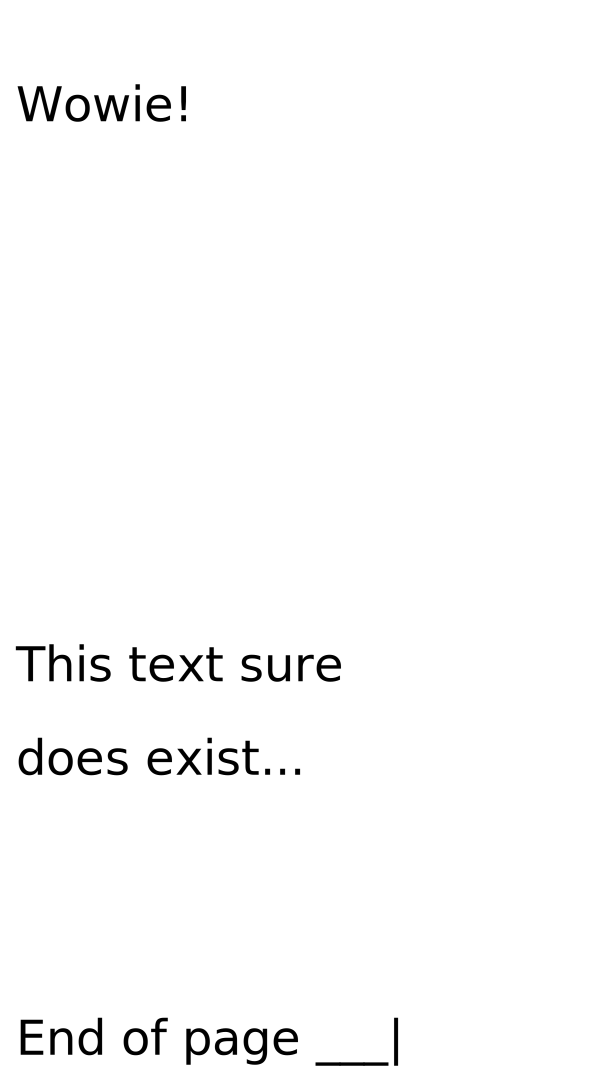
\includegraphics[width=0.8\textwidth]{images/hiv-figure}
            \end{center}
        \end{column}

    \end{columns}

\end{frame}

%--------------------------------------------------
\section{Inferring information from a tree}
%--------------------------------------------------

\begin{frame} \frametitle{\insertsection}

    \begin{columns}

        \begin{column}{0.6\textwidth}
            
            \begin{center}
                \centering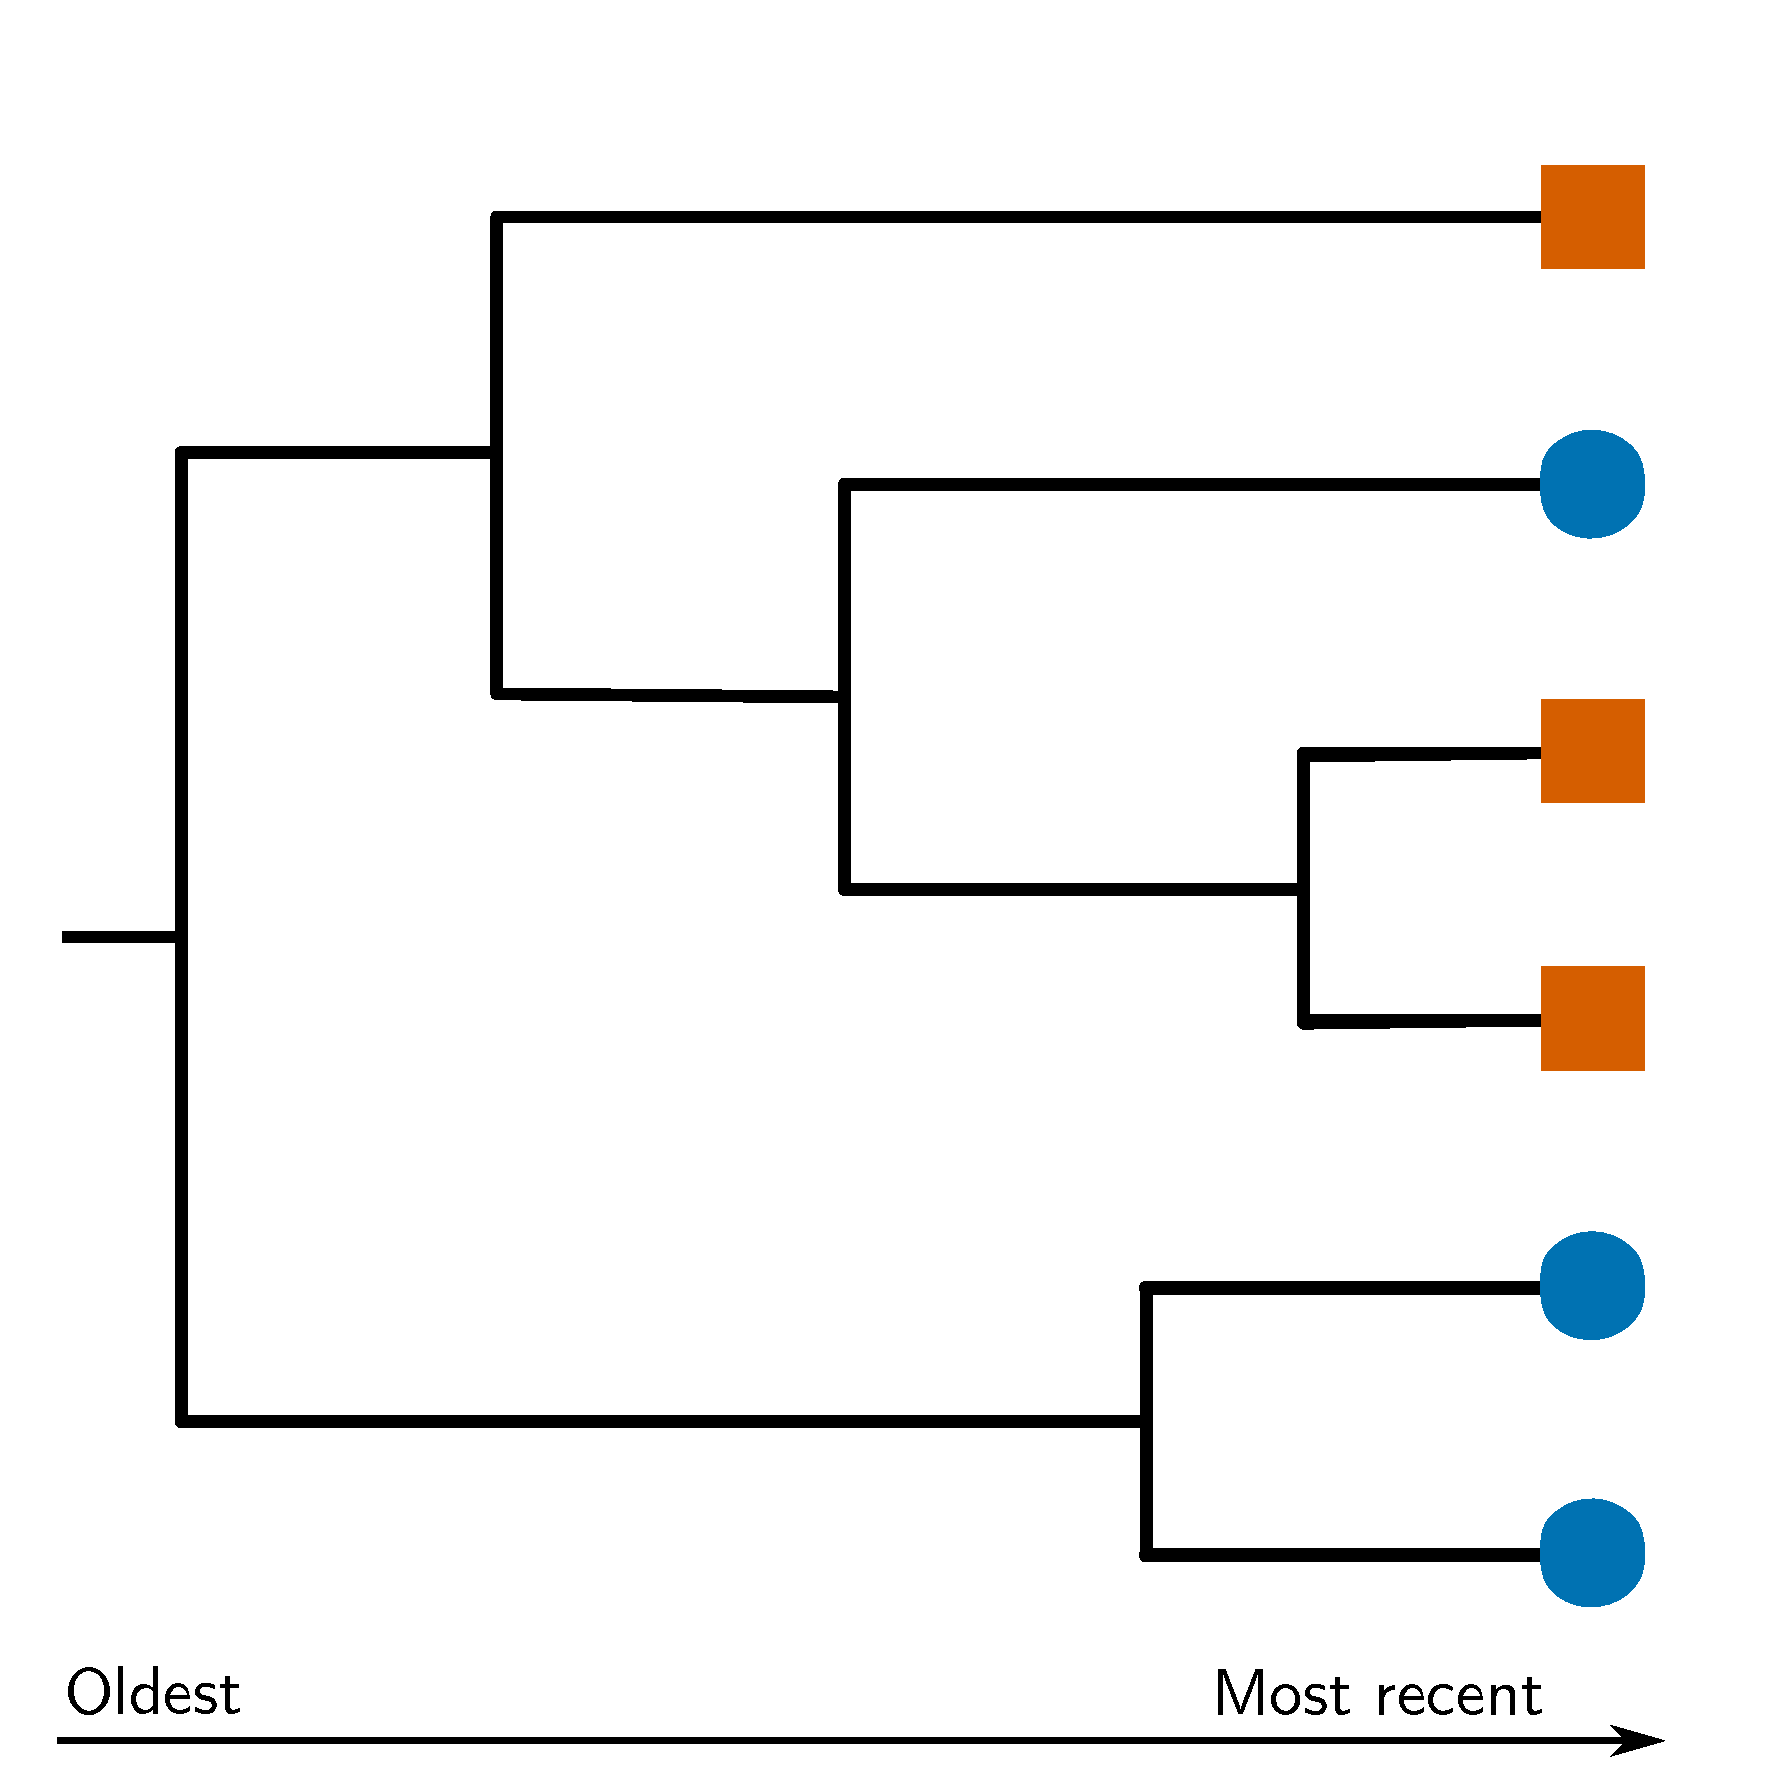
\includegraphics[width=0.8\textwidth]{images/tree-blank}
            \end{center}

        \end{column}

        \begin{column}{0.5\textwidth}

            \begin{itemize}
                \item Tips represent individual viral sequences
                \item Shows the evolutionary distance between individuals
                \item What can we infer about a single transmission time?
            \end{itemize}

        \end{column}

    \end{columns}

\end{frame}

\begin{frame}

    \begin{center}

        \centering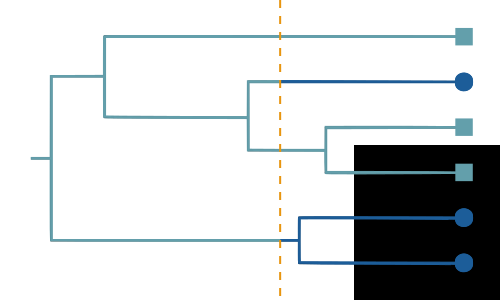
\includegraphics[width=0.8\textwidth]{images/tree-option1}
        
    \end{center}

\end{frame}


\begin{frame}

    \begin{center}

        \centering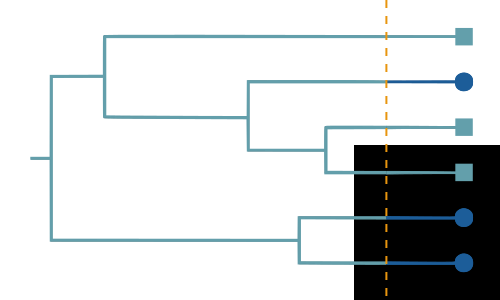
\includegraphics[width=0.8\textwidth]{images/tree-option2}

    \end{center}

\end{frame}


\begin{frame}

    \begin{center}

        \centering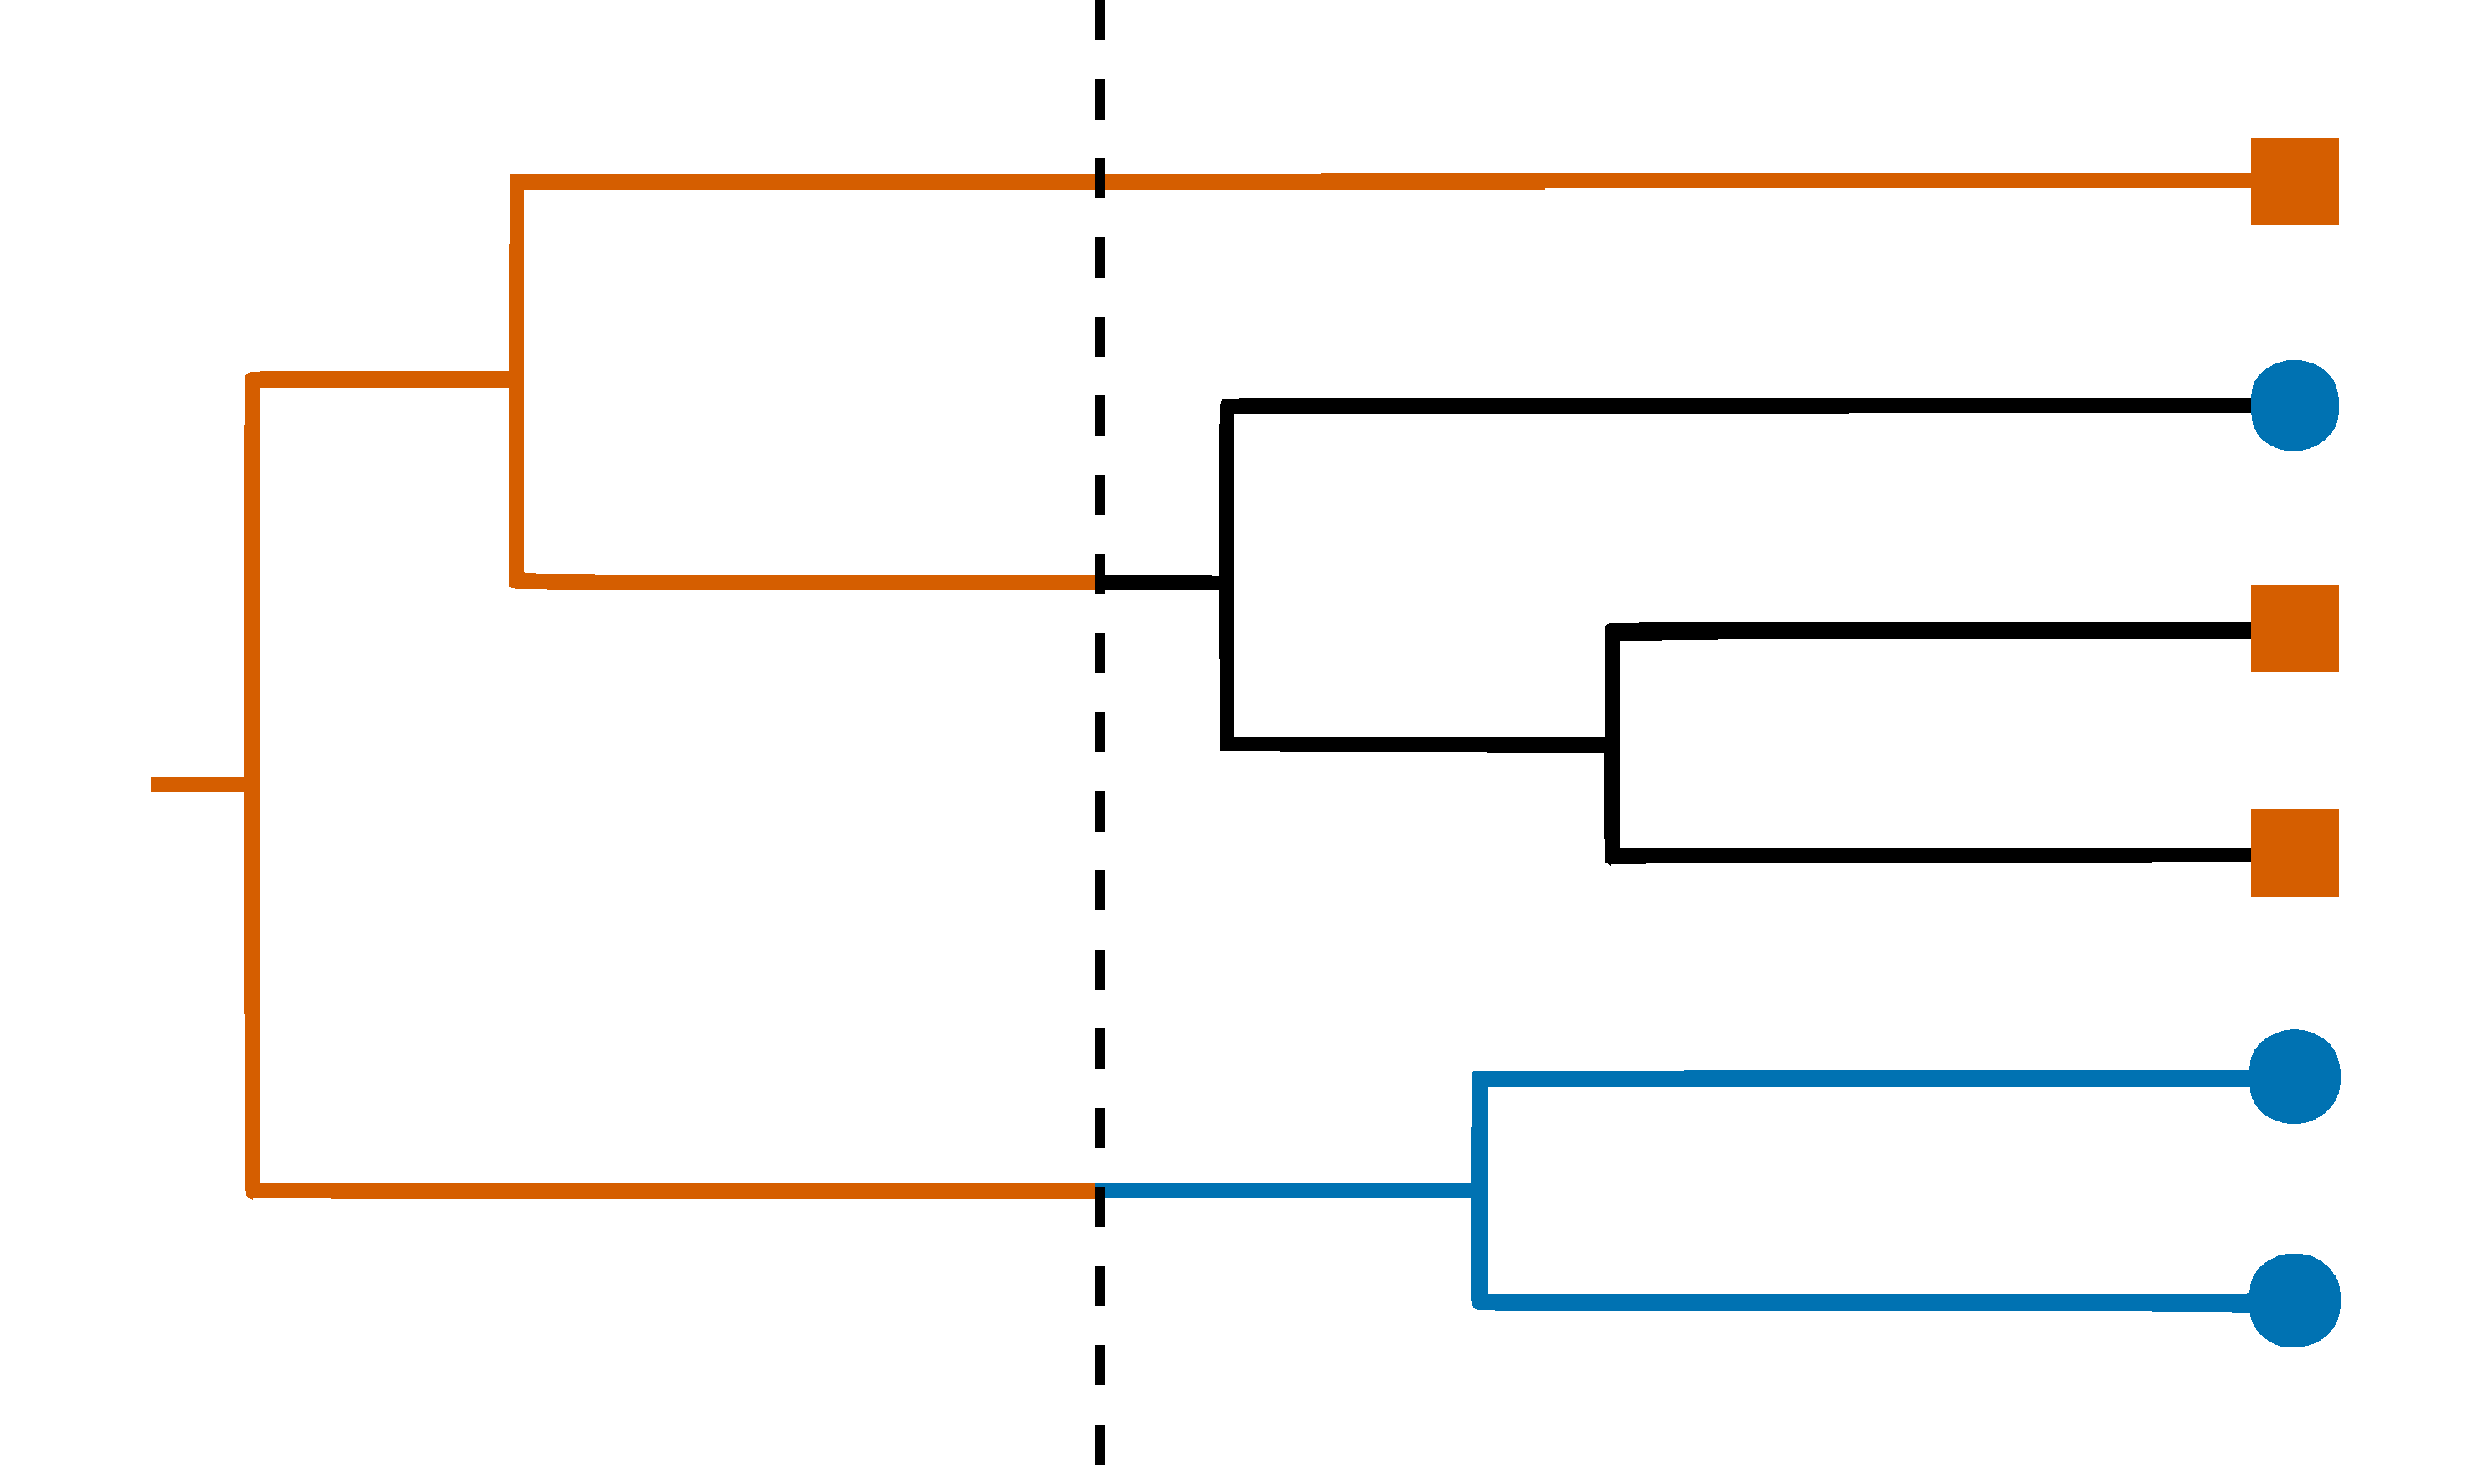
\includegraphics[width=0.8\textwidth]{images/tree-option3}

    \end{center}

\end{frame}

%-------------------------------------------------
\section{Linear population growth (IDK where this should go)}
%-------------------------------------------------

\begin{frame} \frametitle{\insertsection}
    \centering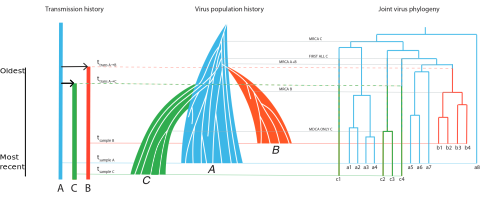
\includegraphics[width=\textwidth]{images/thomas-figure}
\end{frame}

%--------------------------------------------------
\section{Coalescent modeling}
%--------------------------------------------------

\begin{frame} \frametitle{\insertsection}

    Main findings:
    \begin{itemize}
        \item First
        \item Second
    \end{itemize}

\end{frame}

\begin{frame} \frametitle{\insertsection}
    \centering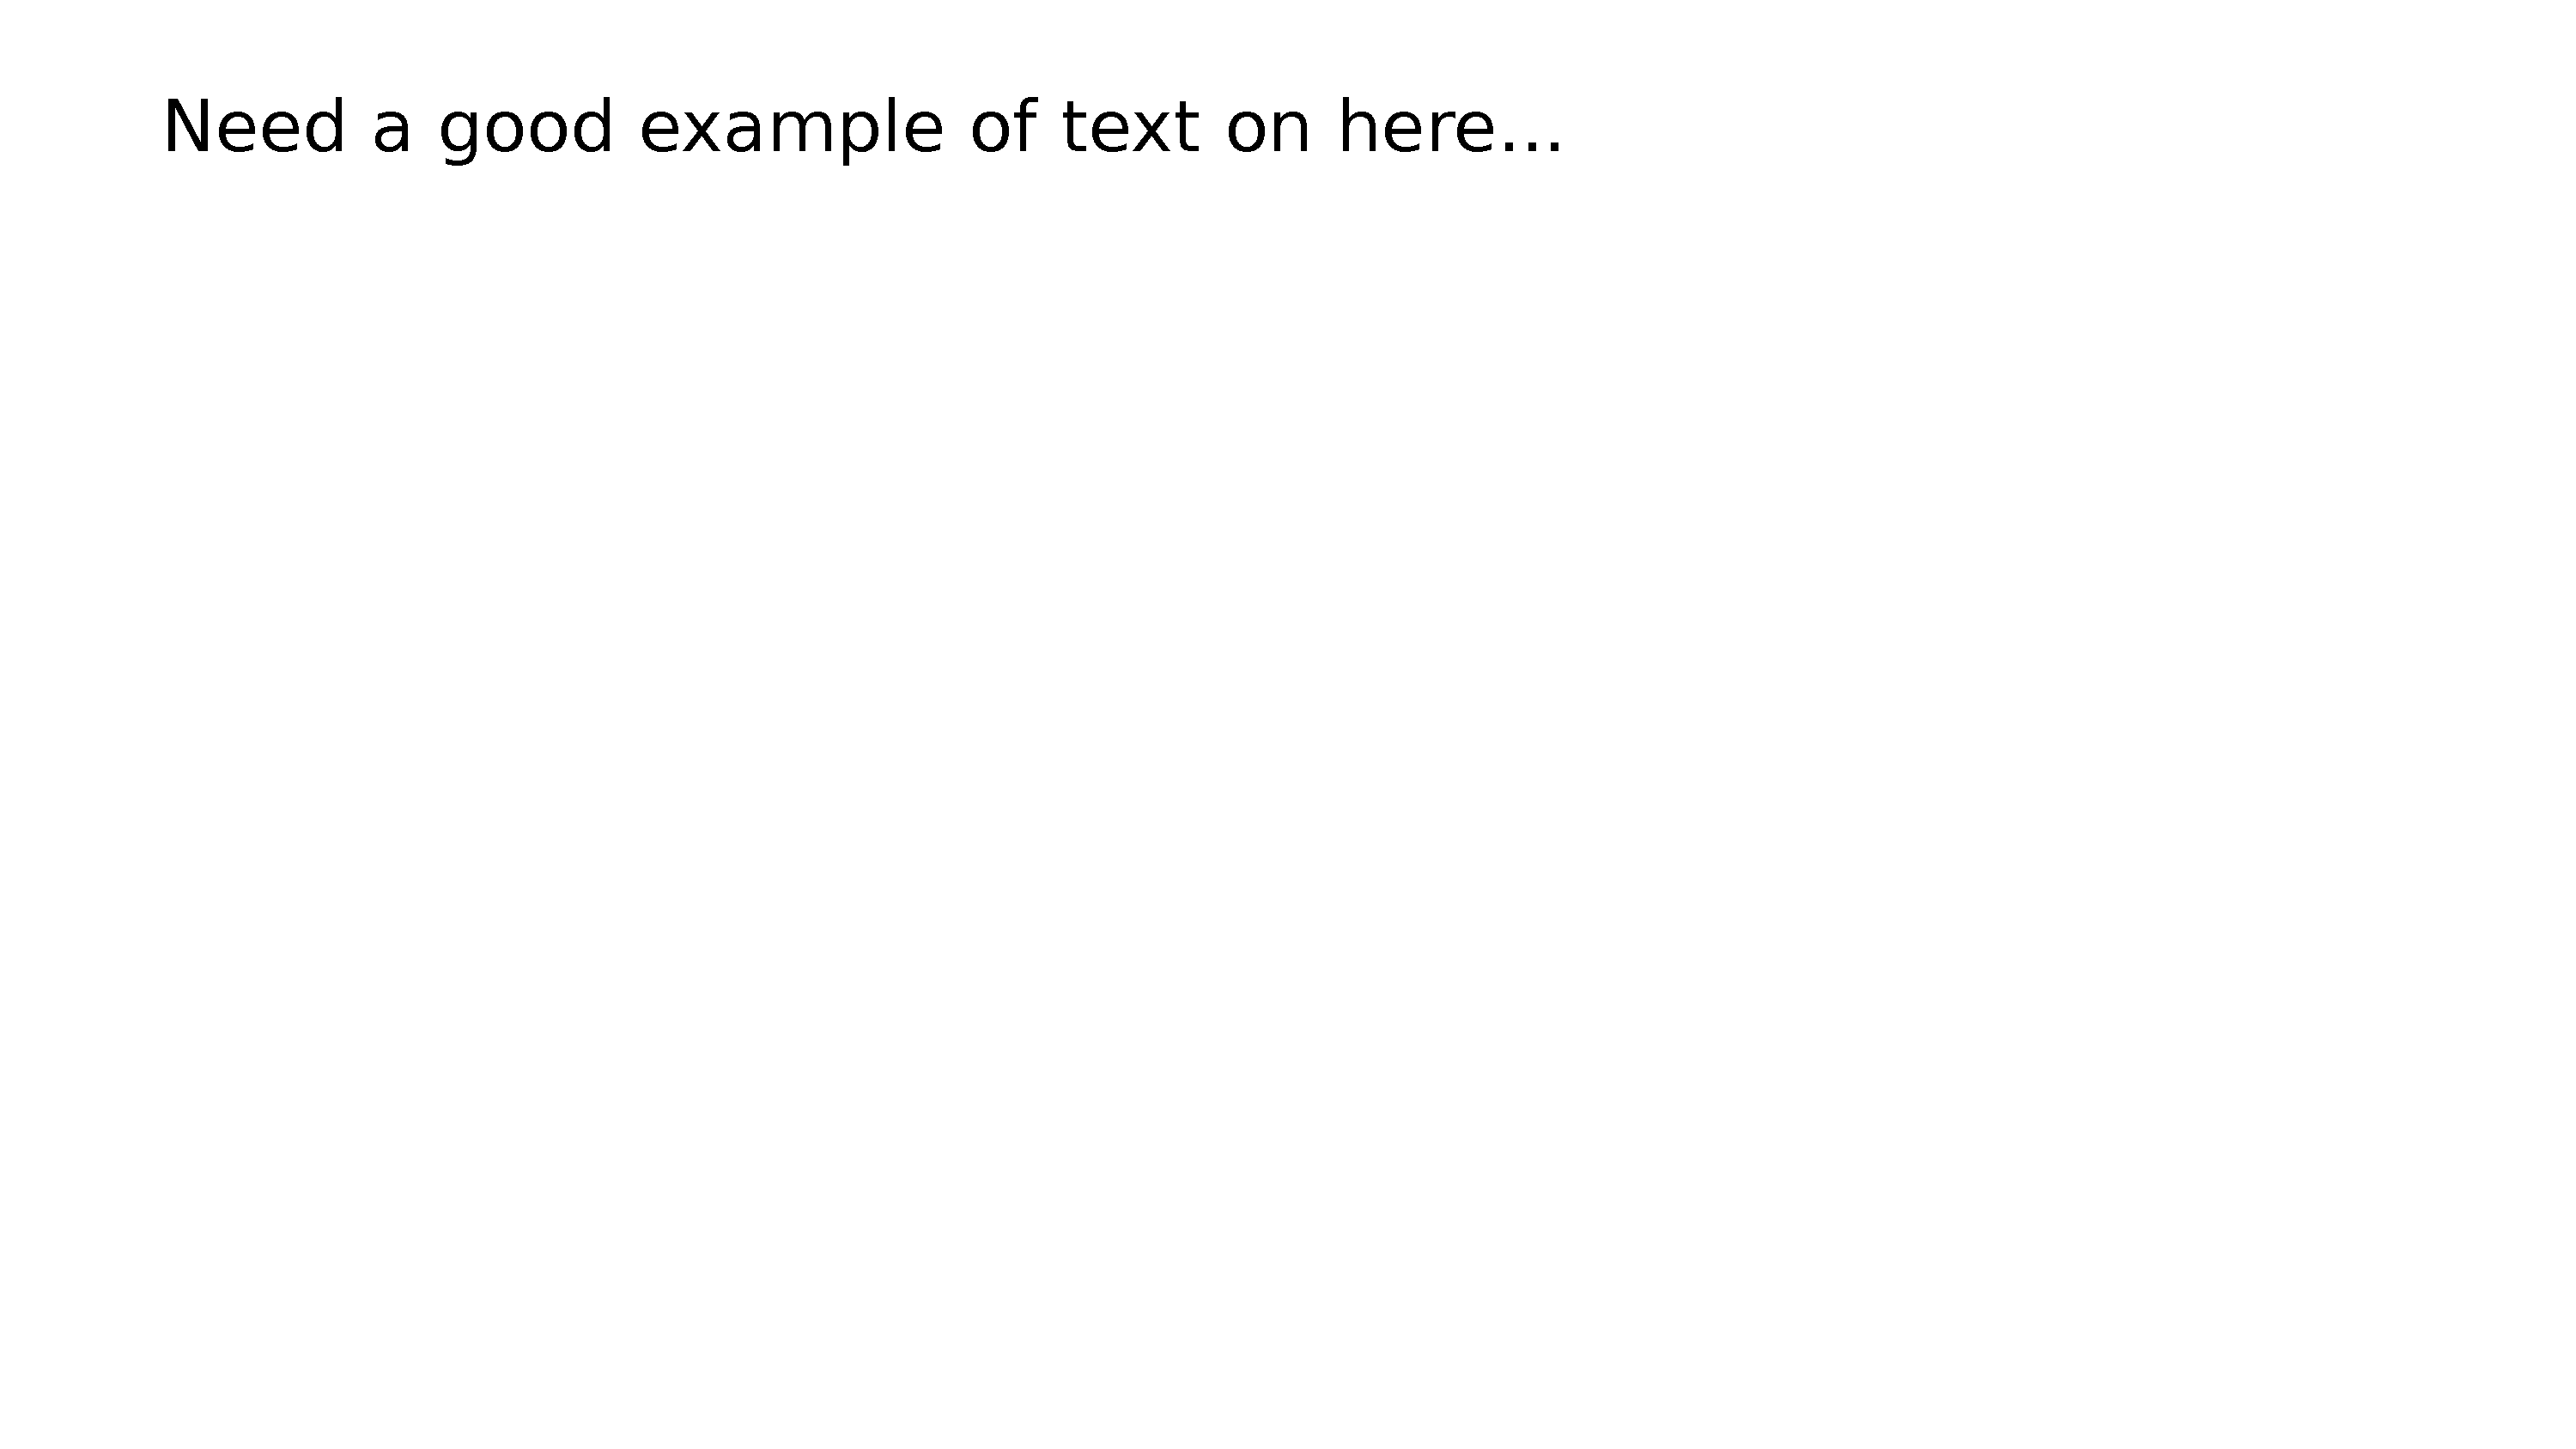
\includegraphics[width=0.8\textwidth]{images/example}
\end{frame}

%--------------------------------------------------
\section{Predictions on a changing population}
%--------------------------------------------------

\begin{frame} \frametitle{\insertsection}

    This is where I plan to put my stuff about
    expanding everything up to a linear model,
    and how it should allow us to make inferences
    based on how the times are changing.

\end{frame}

%--------------------------------------------------
\section{Results}
%--------------------------------------------------

\begin{frame} \frametitle{\insertsection}

    What I did\ldots

\end{frame}

%--------------------------------------------------
\section{Conclusion}
%--------------------------------------------------

\begin{frame} \frametitle{\insertsection}

    Parting thoughts\ldots

\end{frame}

\end{document}
